% Chapter Template

\chapter{Software Design} % Main chapter title

\label{Chapter5} % Change X to a consecutive number; for referencing this chapter elsewhere, use \ref{ChapterX}

\lhead{Chapter 5. \emph{Software Design}} % Change X to a consecutive number; this is for the header on each page - perhaps a shortened title

%----------------------------------------------------------------------------------------
%	SECTION 1
%----------------------------------------------------------------------------------------

\section{Software Architecture}
Software architecture serves as a blueprint for both system and project developing it, defining work assignments that must be carried out by design and implementation teams. The architecture is presented in terms of classes diagram.

%-----------------------------------
%	SUBSECTION 1
%-----------------------------------
\subsection{Overall Class Diagram }

A class diagram is a type of static structure diagram that describes the structure of a system by showing the system's classes, their attributes, operations (or methods), and the relationships among objects. All of system’s structure is shown in Figure \ref{fig:f501}
\begin{figure}[t]
	\centering
	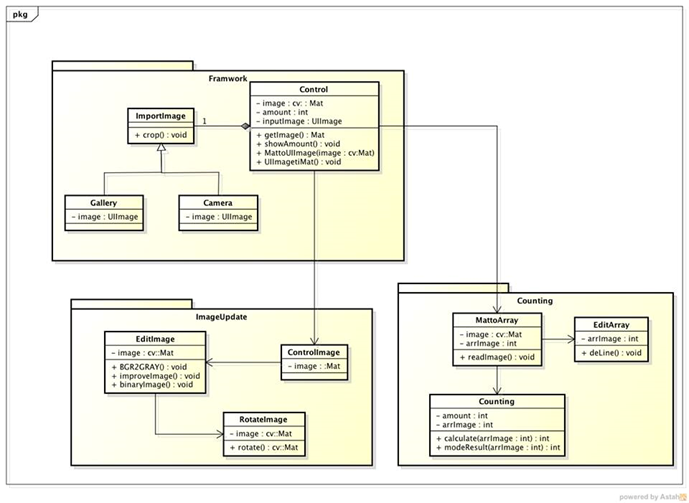
\includegraphics[scale=0.7]{f501.png}
	\caption{Overall class diagram of the application}
	\label{fig:f501}
\end{figure}

The structure of an application consist three packages including \textit{Framework package}, \textit{ImageUpdate package}, and \textit{Counting package}. The framework package functions like an interface class. The package gets an input image and shows final result. An input image will be sent into the ImageUpdate package. The ImageUpdate package is package that preprocessing an image such as image rotation, image conversion, etc. The last package is Counting package. It counts the number of sheets of cloth.
%-----------------------------------
%	SUBSECTION 2
%-----------------------------------
\subsection{Framework Package}
Framework is a package served as user interface part of the application. It gets an image input from user and displays a counting result. The input image can be obtained from image gallery or photographing. The counting result is returned from \textit{MattoArray} class in Counting package. This package has four classes including \textit{Control class}, \textit{Gallery class}, \textit{Camera class} and \textit{ImportImage class}. Control class is a main of application. Gallery class is an input image class from the image gallery and Camera class is an input image class from photography both inherit from ImportImage class. The Framework package is shown in Figure \ref{fig:f502}.
\begin{figure}[t]
	\centering
	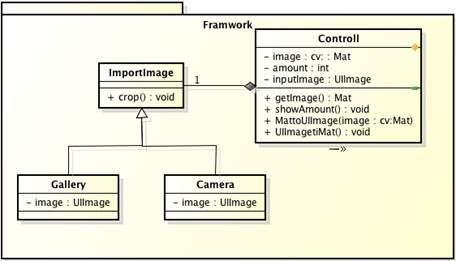
\includegraphics[scale=0.9]{f502.png}
	\caption{Framework package}
	\label{fig:f502}
\end{figure}

%-----------------------------------
%	SUBSECTION 3
%-----------------------------------
\subsection{ImageUpdate Package}
ImageUpdate is a package that pre-processes an image before sending to Counting package. It contains three classes, i.e. \textit{ControllImage class} gets and returns an image to Framework package, \textit{EditImage class} converts an original image to binary image with OpenCV library and \textit{RotateImage class} checks orientation of the sheets of cloth in the image and rotate the image such that the layers of the sheets of cloth align vertically for counting. The ImageUpdate package is shown in Figure \ref{fig:f503}.
\begin{figure}[t]
	\centering
	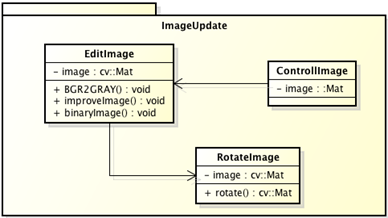
\includegraphics[scale=0.9]{f503.png}
	\caption{ImageUpdate package}
	\label{fig:f503}
\end{figure}

%-----------------------------------
%	SUBSECTION 4
%-----------------------------------
\subsection{Counting Package}
There are three classes in the Counting package, i.e. MattoArray class which received an image and stored intensity value of each pixel to the array, \textit{EditArray class}, which improved the number of intensity value in the array, and Counting class that count number of intensity value in the array count length of the series of 0 or 1. it will be discussed later chapter. The Counting package is shown in Figure \ref{fig:f504}.
\begin{figure}[t]
	\centering
	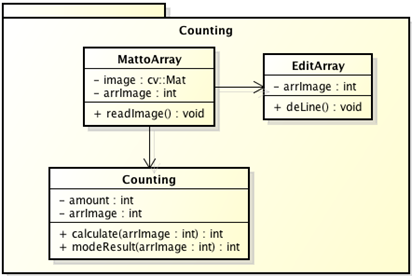
\includegraphics[scale=0.9]{f504.png}
	\caption{Counting package}
	\label{fig:f504}
\end{figure}

All of these presents about software designing of the application thorough.  Explanations, each functions in classes is performed. 
